\documentclass[12pt,a4paper]{article}
\usepackage[margin=1in]{geometry}
\usepackage{graphicx}
\usepackage{amsmath,amssymb}
\usepackage{booktabs}
\usepackage{hyperref}
\usepackage{xcolor}
\usepackage{enumitem}
\usepackage{tikz}
\usetikzlibrary{arrows.meta,positioning,shapes.geometric,fit,calc}
\usepackage{float}
\usepackage{caption}
\usepackage{listings}
\usepackage{fancyhdr}
\usepackage{pifont}
\usepackage{mdframed}
\usepackage{fontawesome5}

\hypersetup{colorlinks=true,linkcolor=blue!60!black,urlcolor=blue!70!black}

\definecolor{layerone}{RGB}{52,152,219}
\definecolor{layertwo}{RGB}{46,204,113}
\definecolor{layerthree}{RGB}{231,76,60}
\definecolor{novelty}{RGB}{155,89,182}
\definecolor{highlight}{RGB}{255,248,220}
\definecolor{greenbox}{RGB}{232,245,233}
\definecolor{redbox}{RGB}{255,235,238}
\definecolor{bluebox}{RGB}{227,242,253}
\definecolor{purplebox}{RGB}{243,229,245}
\definecolor{codebg}{RGB}{245,245,245}

\mdfdefinestyle{keypoint}{
  backgroundcolor=highlight,
  linewidth=2pt,
  linecolor=orange!70!black,
  roundcorner=8pt,
  innertopmargin=10pt,
  innerbottommargin=10pt,
}
\mdfdefinestyle{beforebox}{
  backgroundcolor=redbox,
  linewidth=2pt,
  linecolor=red!60!black,
  roundcorner=8pt,
  innertopmargin=8pt,
  innerbottommargin=8pt,
}
\mdfdefinestyle{afterbox}{
  backgroundcolor=greenbox,
  linewidth=2pt,
  linecolor=green!60!black,
  roundcorner=8pt,
  innertopmargin=8pt,
  innerbottommargin=8pt,
}
\mdfdefinestyle{novelbox}{
  backgroundcolor=purplebox,
  linewidth=2pt,
  linecolor=novelty,
  roundcorner=8pt,
  innertopmargin=8pt,
  innerbottommargin=8pt,
}

\pagestyle{fancy}
\fancyhf{}
\rhead{\small DR Digital Twin --- Complete Explainer}
\lhead{\small Capstone Project}
\cfoot{\thepage}

\title{%
  \vspace{-1cm}
  {\LARGE\bfseries Digital Twin for Diabetic Retinopathy}\\[8pt]
  {\Large A Complete Explanation of the Project}\\[6pt]
  {\large What We Started With, What We Built, and How It All Works}\\[12pt]
  {\normalsize\itshape Capstone Project Explainer}
}
\author{}
\date{\today}

\begin{document}
\maketitle
\thispagestyle{fancy}

\tableofcontents
\newpage

%==========================================================================
\section{The Big Picture: What Is This Project?}
%==========================================================================

\begin{mdframed}[style=keypoint]
\textbf{One-line summary:} We built a computer system that looks at eye scans of diabetic patients, figures out what is wrong, predicts how the disease will change over time, and recommends which medicine will work best --- all in one connected pipeline.
\end{mdframed}

\subsection{The Disease: Diabetic Retinopathy}

Diabetes is a disease where the body cannot properly control blood sugar levels. Over time, high blood sugar damages the tiny blood vessels in the back of the eye (the retina). This damage is called \textbf{Diabetic Retinopathy (DR)}, and it is one of the leading causes of blindness worldwide --- affecting over 100 million people.

Doctors monitor DR by taking special scans of the eye called \textbf{OCT scans} (Optical Coherence Tomography). These are like ultrasound images but for the eye --- they show cross-sections of the retina in very fine detail. In these scans, doctors look for specific signs of damage called \textbf{biomarkers}. Think of biomarkers as ``red flags'' that tell the doctor how bad the disease is and what kind of treatment might help.

\subsection{The Six Biomarkers We Detect}

Our system looks for six specific biomarkers in each OCT scan:

\begin{table}[H]
\centering
\caption{The six retinal biomarkers our system detects.}
\small
\begin{tabular}{@{}lll@{}}
\toprule
\textbf{Short Name} & \textbf{Full Name} & \textbf{What It Means} \\
\midrule
IRHRF & Intraretinal Hyperreflective Foci & Bright dots = inflammation or hard deposits \\
PAVF & Partially Attached Vitreous Face & The jelly in the eye is partially peeling away \\
FAVF & Fully Attached Vitreous Face & The jelly in the eye is still fully attached \\
IRF & Intraretinal Fluid & Fluid-filled pockets inside the retina \\
DRT/ME & Diffuse Retinal Thickening & The retina is swollen (macular edema) \\
VD & Vitreous Debris & Floating particles in the eye jelly \\
\bottomrule
\end{tabular}
\end{table}

Each biomarker is either \textbf{present} (active) or \textbf{absent} in a given scan. A patient with many active biomarkers is in worse shape than one with few.

\subsection{The Dataset: OLIVES}

All our data comes from a real, published clinical dataset called \textbf{OLIVES} (Ophthalmic Labels for Investigating Visual Eye Semantics). This is not simulated or made-up data --- it comes from actual patients in actual clinical trials.

\begin{itemize}[nosep]
  \item \textbf{9,396 eye scan images} from \textbf{87 real patients}
  \item Each image is labeled by doctors: which of the 6 biomarkers are present
  \item Patients were scanned \textbf{multiple times} over the course of treatment (longitudinal data)
  \item Two clinical trials: PRIME and TREX DME (both testing anti-VEGF drugs)
  \item Also includes clinical measurements: visual acuity (how well they see) and retinal thickness
\end{itemize}

\textbf{We use zero synthetic or simulated data. Everything in our system comes from real patients.}

\subsection{What Is a ``Digital Twin''?}

A \textbf{digital twin} is a computer model of a real-world thing. In manufacturing, a digital twin of a jet engine lets engineers test ``what if we increase the temperature?'' without risking a real engine. In our case:

\begin{mdframed}[style=keypoint]
A \textbf{patient digital twin} is a computer model of a specific patient's eye disease. It lets doctors ask ``what if we give this patient Drug~A vs.\ Drug~B?'' and see predicted outcomes \emph{before} actually giving the treatment.
\end{mdframed}

Our digital twin takes a patient's eye scans, builds a model of their disease state, predicts how the disease will progress over future visits, and simulates what different treatments would do.


%==========================================================================
\section{The Two Original Projects (What They Had)}
%==========================================================================

This project started by combining two separate capstone projects. Neither project alone was complete --- each had a piece of the puzzle.

\subsection{Project A: The Proposal (SVM10)}

\textbf{Title:} ``Virtual Drug Testing for Diabetic Retinopathy Using Digital Twins''

\begin{mdframed}[style=beforebox]
\textbf{What Project A had:}
\begin{itemize}[nosep]
  \item A written proposal document (like a plan on paper)
  \item The \emph{idea} of building a digital twin for eye disease
  \item A literature review (summary of what other researchers have done)
  \item Block diagrams showing a three-layer architecture concept
  \item A suggestion to use ``PINNs'' (Physics-Informed Neural Networks) for modeling
\end{itemize}

\textbf{What Project A did NOT have:}
\begin{itemize}[nosep]
  \item No Python code --- not a single line
  \item No trained models
  \item No dataset integration
  \item No working prototype
  \item No results, no metrics, no experiments
  \item The PINN approach it suggested does not actually work for this problem (PINNs solve continuous equations, but biomarkers are binary --- either present or not)
\end{itemize}
\end{mdframed}

\textbf{In simple terms:} Project~A was a well-written plan, but only a plan. It was like having architectural blueprints for a house, but no bricks, no workers, and some of the blueprint's ideas were not structurally possible.

\subsection{Project B: The Notebook}

\textbf{Title:} ``Biomarker Co-occurrence Prediction Using Graph Neural Networks on OCT Scans''

\begin{mdframed}[style=beforebox]
\textbf{What Project B had:}
\begin{itemize}[nosep]
  \item Three working Jupyter notebooks ($\sim$200 code cells)
  \item A trained AI model (Prior-GAT) that can look at an eye scan and detect which biomarkers are present
  \item An NPMI co-occurrence graph (a mathematical way to say ``these biomarkers tend to appear together'')
  \item Four different model variants tested and compared
  \item Real results: F1 scores and AUROC metrics
  \item Proper evaluation: patient-level data splits (no cheating), bootstrap confidence intervals
\end{itemize}

\textbf{What Project B did NOT have:}
\begin{itemize}[nosep]
  \item No modular code structure --- everything was in messy notebooks
  \item Only did ONE task: detecting biomarkers from a single scan
  \item No disease progression modeling (cannot predict future visits)
  \item No treatment simulation (cannot compare drugs)
  \item No causal analysis (cannot answer ``does biomarker A cause biomarker B?'')
  \item No user interface
  \item No way to run the code as a command-line tool
\end{itemize}
\end{mdframed}

\textbf{In simple terms:} Project~B was a working engine, but only one engine. It could look at an eye scan and say ``this patient has IRF and DRT/ME.'' But it could not predict what would happen next week, or which treatment would help. And the code was messy --- all tangled together in notebooks instead of clean, organized files.


%==========================================================================
\section{What We Built (The Unified System)}
%==========================================================================

We took the \emph{idea} from Project~A and the \emph{working detection engine} from Project~B, and built a complete system from the ground up.

\begin{mdframed}[style=afterbox]
\textbf{What the unified system does:}
\begin{enumerate}[nosep]
  \item \textbf{Detects biomarkers} from eye scans (kept from Project B, upgraded)
  \item \textbf{Predicts disease progression} over future visits (completely new)
  \item \textbf{Simulates different treatments} and recommends the best one (completely new)
  \item \textbf{Discovers causal relationships} between biomarkers (completely new --- this is the main novelty)
  \item \textbf{Shows everything} in an interactive dashboard (completely new)
  \item \textbf{Monitors everything} via a Grafana analytics dashboard (completely new)
\end{enumerate}
\end{mdframed}


%==========================================================================
\section{How the System Works: Three Layers}
%==========================================================================

The system is organized as a three-layer pipeline. Each layer does one job and passes its output to the next layer.

\begin{figure}[H]
\centering
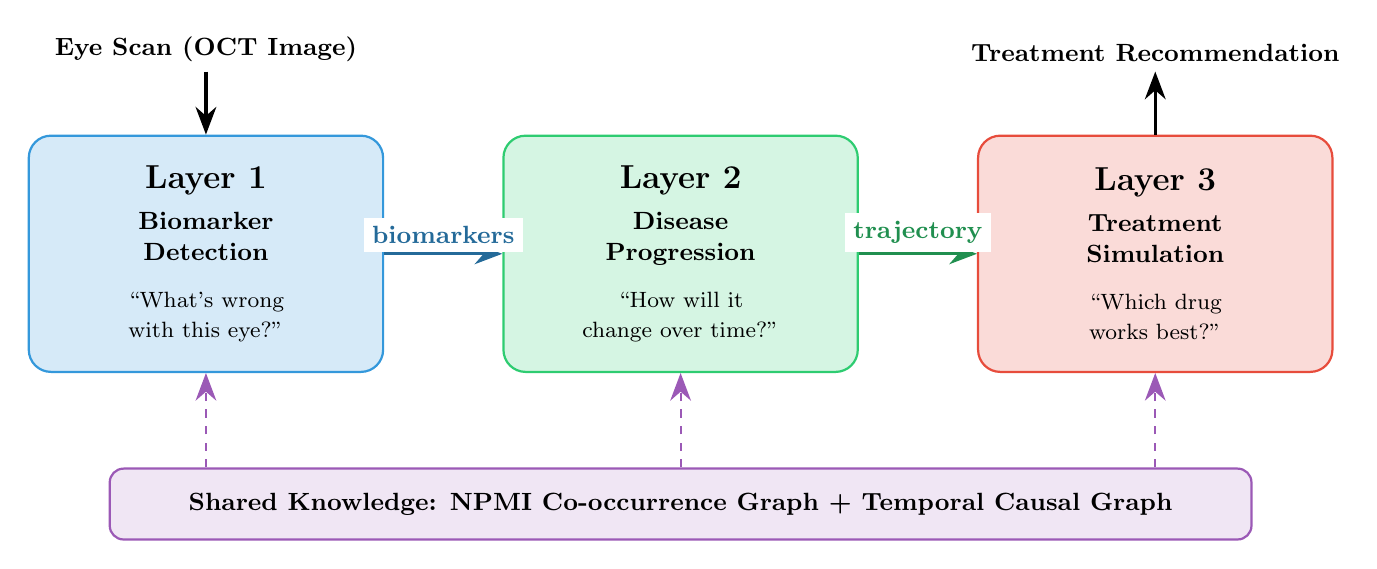
\begin{tikzpicture}[
  layer/.style={draw, rounded corners=8pt, minimum width=4.5cm, minimum height=3cm, align=center, font=\small, thick},
  arrow/.style={-{Stealth[length=10pt]}, very thick},
  label/.style={font=\footnotesize\bfseries, fill=white, inner sep=3pt},
]
  \node[layer, fill=layerone!20, draw=layerone] (l1) {
    \textbf{\large Layer 1}\\[4pt]
    \textbf{Biomarker}\\
    \textbf{Detection}\\[6pt]
    \footnotesize ``What's wrong\\
    \footnotesize with this eye?''
  };

  \node[layer, fill=layertwo!20, draw=layertwo, right=1.5cm of l1] (l2) {
    \textbf{\large Layer 2}\\[4pt]
    \textbf{Disease}\\
    \textbf{Progression}\\[6pt]
    \footnotesize ``How will it\\
    \footnotesize change over time?''
  };

  \node[layer, fill=layerthree!20, draw=layerthree, right=1.5cm of l2] (l3) {
    \textbf{\large Layer 3}\\[4pt]
    \textbf{Treatment}\\
    \textbf{Simulation}\\[6pt]
    \footnotesize ``Which drug\\
    \footnotesize works best?''
  };

  \draw[arrow, layerone!70!black] (l1) -- node[label, above] {\small biomarkers} (l2);
  \draw[arrow, layertwo!70!black] (l2) -- node[label, above] {\small trajectory} (l3);

  % NPMI bar
  \node[draw, rounded corners=5pt, fill=novelty!15, draw=novelty, minimum width=14.5cm, minimum height=0.9cm, below=1.2cm of l2, font=\small\bfseries, thick] (npmi) {Shared Knowledge: NPMI Co-occurrence Graph + Temporal Causal Graph};

  \draw[arrow, dashed, novelty, thick] (npmi.north -| l1) -- (l1.south);
  \draw[arrow, dashed, novelty, thick] (npmi.north -| l2) -- (l2.south);
  \draw[arrow, dashed, novelty, thick] (npmi.north -| l3) -- (l3.south);

  % Input/Output
  \node[above=0.8cm of l1, font=\small\bfseries] (input) {Eye Scan (OCT Image)};
  \node[above=0.8cm of l3, font=\small\bfseries] (output) {Treatment Recommendation};
  \draw[arrow] (input) -- (l1.north);
  \draw[arrow] (l3.north) -- (output);
\end{tikzpicture}
\caption{The three-layer pipeline. An eye scan goes in, a treatment recommendation comes out.}
\end{figure}


\subsection{Layer 1: Biomarker Detection --- ``What's Wrong With This Eye?''}

\textbf{The job:} Take an OCT scan image and determine which of the 6 biomarkers are present.

\textbf{How it works, step by step:}

\begin{enumerate}
  \item \textbf{The image goes in.} A grayscale OCT scan (224$\times$224 pixels, or 384$\times$384 in high-performance mode) is fed into the system.

  \item \textbf{A neural network extracts features.} We use a pretrained ResNet-18 --- a well-known image recognition model originally trained on millions of everyday photos. We fine-tune it on eye scans. It converts the image into a list of 512 numbers (a ``feature vector'') that capture the important patterns in the scan.

  \item \textbf{Features are split into 6 biomarker nodes.} The 512 numbers are reshaped into 6 separate representations --- one for each biomarker. Each representation is 128 numbers long (256 in high-performance mode).

  \item \textbf{A Graph Neural Network refines the predictions.} This is where it gets clever. We know from the data that certain biomarkers tend to appear together. For example, IRF (fluid in the retina) and DRT/ME (retinal swelling) have an NPMI score of +0.661, meaning they very often co-occur --- which makes medical sense, since fluid causes swelling. We also know that PAVF and FAVF have an NPMI of $-0.774$, meaning they almost never appear together --- because the vitreous jelly cannot be both partially and fully attached at the same time.

  This knowledge is encoded in a graph, and our \textbf{Prior-GAT} (Prior Graph Attention Network) uses it to refine predictions. If the model detects IRF, the graph connection nudges it to also look more carefully for DRT/ME. The key formula is:
  \[
  \text{attention}(i, j) = \text{softmax}\!\left(\frac{Q_i \cdot K_j}{\sqrt{d}} + \lambda \cdot \text{NPMI}(i,j)\right)
  \]
  The $\lambda$ is a learnable number that the model adjusts during training --- it decides how much to trust the known relationships vs.\ what it learns from the data.

  \item \textbf{Six yes/no predictions come out.} For each biomarker, the model outputs a probability (0 to 1). We use optimized thresholds (not just 0.5) to decide ``present'' vs.\ ``absent.''
\end{enumerate}

\textbf{We train four model variants} and compare them:

\begin{table}[H]
\centering
\small
\begin{tabular}{@{}llp{7cm}@{}}
\toprule
\textbf{Model} & \textbf{Uses Graph?} & \textbf{How It Works} \\
\midrule
CNN Baseline & No & Just the image features, no biomarker relationships \\
GCN & Yes (positive only) & Uses co-occurrence relationships between biomarkers \\
Signed GCN & Yes (positive + negative) & Also uses mutual exclusivity (e.g., PAVF vs FAVF) \\
\textbf{Prior-GAT} & \textbf{Yes (full, learnable)} & \textbf{Best model. Uses attention + NPMI bias with a learnable weight} \\
\bottomrule
\end{tabular}
\end{table}

\textbf{Training details:}
\begin{itemize}[nosep]
  \item Patients are split 60/20/20 into train/validation/test sets, at the patient level (all scans from one patient go into the same set, so the model cannot cheat by seeing the same patient in training and testing)
  \item We train with 3 random seeds (5 in high-performance mode) and report average results
  \item We use class-weighted loss (because some biomarkers are rare)
  \item Mixed-precision training (faster on GPU), gradient clipping (prevents training explosions), early stopping (prevents overfitting)
\end{itemize}

%---

\subsection{Layer 2: Disease Progression --- ``How Will It Change Over Time?''}

\textbf{The job:} Given a patient's history of biomarker states across multiple visits, predict what their biomarkers will look like at the next visit.

\textbf{Why this matters:} A doctor does not just want to know ``this patient has IRF today.'' They want to know ``will this patient still have IRF in 3 months? Will new biomarkers appear?''

\textbf{How it works:}

\begin{enumerate}
  \item \textbf{Extract real patient sequences from OLIVES.} Many patients in OLIVES were scanned multiple times. We extract their biomarker history: visit 1 biomarkers, visit 2 biomarkers, visit 3 biomarkers, etc.

  \item \textbf{Feed sequences into an LSTM.} An LSTM (Long Short-Term Memory) is a type of neural network designed for sequential data. It reads the biomarker history one visit at a time and learns patterns like ``patients who have IRF at visit 1 tend to develop DRT/ME by visit 3.''

  \item \textbf{The Graph-Constrained LSTM} (our best model) adds an extra step: after the LSTM makes its prediction, the prediction is refined using the same NPMI graph from Layer~1. This ensures the model's predictions respect known biomarker relationships. If it predicts IRF will be present, the graph nudges it to also predict DRT/ME.

  \item \textbf{Output:} Predicted biomarker probabilities for the next visit.
\end{enumerate}

\textbf{Three model variants:}
\begin{itemize}[nosep]
  \item \textbf{ProgressionLSTM} --- plain LSTM, no graph
  \item \textbf{GraphConstrainedProgressionLSTM} --- LSTM + NPMI graph refinement (best)
  \item \textbf{ProgressionTransformer} --- transformer-based model with attention over the visit sequence
\end{itemize}

%---

\subsection{Layer 3: Treatment Simulation --- ``Which Drug Works Best?''}

\textbf{The job:} For a given patient, simulate what would happen under four different treatments and recommend the best one.

\textbf{The four treatments:}
\begin{enumerate}[nosep]
  \item \textbf{Anti-VEGF} --- injections that block blood vessel growth (most common DR treatment)
  \item \textbf{Steroid} --- anti-inflammatory injections
  \item \textbf{Laser photocoagulation} --- using a laser to seal leaking blood vessels
  \item \textbf{Observation} --- no treatment, just monitoring (the baseline)
\end{enumerate}

\textbf{How it works:}

\begin{enumerate}
  \item \textbf{Take the patient's current state} (which biomarkers are active, their clinical measurements).

  \item \textbf{Pick a treatment.} Each treatment is represented as a learned embedding (a vector of numbers the model learns during training that captures the treatment's identity).

  \item \textbf{Roll forward the progression model} step by step. Use the Layer~2 model to predict visit~2, then feed visit~2's prediction back in to predict visit~3, and so on, for $H$ future visits (the ``prediction horizon'').

  \item \textbf{Repeat 50 times with randomness} (Monte Carlo simulation). Each time, the model's dropout layers introduce slight randomness, giving slightly different predictions. This gives us:
    \begin{itemize}[nosep]
      \item The \textbf{average} predicted trajectory (most likely outcome)
      \item A \textbf{95\% confidence interval} (range of plausible outcomes)
      \item \textbf{Uncertainty} at each future visit
    \end{itemize}

  \item \textbf{Do this for all 4 treatments.} Now we have 4 predicted futures.

  \item \textbf{Compare and recommend.} The treatment that results in the lowest final severity score (fewest active biomarkers) is recommended.
\end{enumerate}

\begin{mdframed}[style=keypoint]
\textbf{Example output:} ``For Patient \#42, anti-VEGF reduces severity from 0.67 to 0.23 (best), steroid reduces to 0.35, laser reduces to 0.41, observation stays at 0.65. \textbf{Recommendation: anti-VEGF.}''
\end{mdframed}


%==========================================================================
\section{The Core Novelty: Temporal Causal Biomarker Graph}
%==========================================================================

\begin{mdframed}[style=novelbox]
\textbf{This is the main new contribution of the project} --- something no one has done before for retinal biomarkers. Everything else (detection, progression, simulation) builds on known techniques. The Temporal Causal Biomarker Graph is genuinely novel.
\end{mdframed}

\subsection{The Problem with Regular Co-occurrence}

Layer 1's NPMI graph tells us: ``IRF and DRT/ME tend to appear together (NPMI = +0.661).''

But this does not answer the important questions:

\begin{itemize}
  \item \textbf{Which causes which?} Does IRF cause DRT/ME? Or does DRT/ME cause IRF? Or both?
  \item \textbf{Does the relationship change over time?} Maybe IRF at visit~1 leads to DRT/ME at visit~3, but not the other way around.
  \item \textbf{Do treatments change the relationship?} Maybe anti-VEGF breaks the link between IRF and DRT/ME.
\end{itemize}

NPMI is \emph{undirected} (A $\leftrightarrow$ B) and \emph{static} (one number for all time). We need something \emph{directed} (A $\to$ B) and \emph{temporal} (visit $t$ to visit $t{+}1$).

\subsection{What We Built}

\textbf{Step 1: Directed Temporal Transitions.} For every pair of biomarkers $(i, j)$, we ask: ``When biomarker $i$ is active at visit $t$, how likely is biomarker $j$ to be active at visit $t{+}1$?'' Then we subtract the baseline: ``How likely is $j$ at visit $t{+}1$ when $i$ is \emph{not} active at visit $t$?''

The difference is the \textbf{causal effect}:
\[
\text{CausalEffect}(i \to j) = P(j_{t+1} = 1 \mid i_t = 1) - P(j_{t+1} = 1 \mid i_t = 0)
\]

A positive number means: ``Having biomarker $i$ today makes biomarker $j$ more likely tomorrow.'' A negative number means the opposite. And importantly, $\text{CausalEffect}(\text{IRF} \to \text{DRT/ME})$ can be different from $\text{CausalEffect}(\text{DRT/ME} \to \text{IRF})$ --- the relationship can be asymmetric.

\textbf{Step 2: Treatment-Conditioned Causal Graphs.} We repeat the above calculation separately for each treatment group. This reveals how treatments change the causal structure:

\begin{itemize}[nosep]
  \item Under \textbf{observation}: IRF $\to$ DRT/ME has effect $+0.15$ (fluid drives swelling)
  \item Under \textbf{anti-VEGF}: IRF $\to$ DRT/ME has effect $+0.03$ (drug blocks the link)
\end{itemize}

This is clinically powerful: it tells the doctor exactly which disease pathways a treatment interrupts.

\textbf{Step 3: Statistical Testing.} We use a Granger-style causality test (chi-squared contingency test) to determine which causal links are statistically significant ($p < 0.05$) and not just random noise.

\textbf{Step 4: Causal Chain Discovery.} We search for multi-hop pathways:
\[
\text{IRF} \xrightarrow{+0.144} \text{DRT/ME} \xrightarrow{+0.118} \text{IRF}
\]
This is a \textbf{feedback loop}: IRF causes DRT/ME, which in turn causes more IRF. This suggests that early treatment of IRF could break the cycle and prevent escalation.

\textbf{Step 5: Interventional Analysis.} Given the causal graph, we can estimate: ``If we could magically remove IRF (via treatment), what would happen to all other biomarkers?'' We calculate both direct effects (IRF $\to$ DRT/ME) and indirect effects (IRF $\to$ VD $\to$ DRT/ME through intermediate biomarkers).


\subsection{Why This Is New}

\begin{table}[H]
\centering
\caption{What existing methods can and cannot do.}
\begin{tabular}{@{}lcccc@{}}
\toprule
\textbf{Method} & \textbf{Directed?} & \textbf{Temporal?} & \textbf{Treatment-} & \textbf{Can answer} \\
 & & & \textbf{conditioned?} & \textbf{``what if?''} \\
\midrule
NPMI (Project B) & \ding{55} & \ding{55} & \ding{55} & \ding{55} \\
Bayesian networks & \checkmark & \ding{55} & \ding{55} & \ding{55} \\
Granger causality & \checkmark & \checkmark & \ding{55} & \ding{55} \\
\textbf{Our Causal Graph} & \checkmark & \checkmark & \checkmark & \checkmark \\
\bottomrule
\end{tabular}
\end{table}

No previous work has built treatment-conditioned directed causal graphs between retinal biomarkers using real patient data.


%==========================================================================
\section{How We Combined the Two Projects}
%==========================================================================

Here is exactly what came from where:

\begin{table}[H]
\centering
\caption{Origin of each component in the final system.}
\small
\begin{tabular}{@{}lll@{}}
\toprule
\textbf{Component} & \textbf{Origin} & \textbf{What We Did} \\
\midrule
Three-layer architecture idea & Project A & Kept the concept, replaced the technical approach \\
Treatment categories & Project A & Kept (anti-VEGF, steroid, laser, observation) \\
ResNet-18 backbone & Project B & Kept, moved from notebook to module \\
NPMI co-occurrence graph & Project B & Kept, extended with temporal causal version \\
Prior-GAT model & Project B & Kept, moved from notebook to module \\
Training protocol & Project B & Kept, added history logging for Grafana \\
Evaluation methodology & Project B & Kept (bootstrap CI, patient-level splits) \\
\addlinespace
Modular codebase & \textbf{New} & Refactored 200 notebook cells into 7 packages \\
CLI entry point & \textbf{New} & \texttt{run\_pipeline.py} with argument parsing \\
Layer 2: Progression models & \textbf{New} & LSTM, Graph-LSTM, Transformer \\
Layer 2: Causal graph & \textbf{New} & Temporal Causal Biomarker Graph \\
Layer 3: Treatment simulator & \textbf{New} & Counterfactual rollout + Monte Carlo \\
Digital Twin class & \textbf{New} & \texttt{PatientDigitalTwin} tying all layers \\
Streamlit dashboard & \textbf{New} & 5 interactive tabs \\
Grafana dashboard & \textbf{New} & 15 data panels + metrics server \\
Workstation optimization & \textbf{New} & RTX 5090 / i9 Ultra mode \\
Windows batch scripts & \textbf{New} & One-click run scripts \\
\bottomrule
\end{tabular}
\end{table}

\begin{mdframed}[style=keypoint]
\textbf{Summary:} From Project~A we kept the \emph{vision}. From Project~B we kept the \emph{detection engine}. Everything else --- progression modeling, treatment simulation, causal analysis, the dashboard, the Grafana monitoring, the modular codebase --- we built from scratch.
\end{mdframed}


%==========================================================================
\section{The Interactive Dashboard (Streamlit)}
%==========================================================================

The system comes with a beautiful interactive dashboard built with Streamlit. It has 5 tabs:

\begin{enumerate}
  \item \textbf{Current State} --- Shows a radar chart of the patient's biomarker probabilities, highlights which biomarkers are active, explains co-occurrence relationships, and gives a severity score.

  \item \textbf{Disease Progression} --- Lets you pick a treatment and see charts of how each biomarker's probability changes over future visits. Includes uncertainty bands showing the range of possible outcomes.

  \item \textbf{Treatment Comparison} --- Shows all 4 treatments side by side. Bar charts comparing final severity, trajectory lines showing how treatments diverge over time, and a highlighted recommendation.

  \item \textbf{Causal Graph} --- The novel tab. Shows the $6 \times 6$ causal effect heatmap, a directed graph visualization, treatment-conditioned matrices, discovered causal chains, and an interactive ``what-if'' tool where you select a biomarker to ``block'' and see downstream effects.

  \item \textbf{Patient Report} --- Complete summary of everything, exportable as JSON for clinical systems.
\end{enumerate}


%==========================================================================
\section{The Grafana Analytics Dashboard}
%==========================================================================

On top of the Streamlit UI (which is for exploring individual patients), we also built a \textbf{Grafana dashboard} for monitoring the overall system.

\textbf{What is Grafana?} It is an open-source tool used in industry for real-time monitoring dashboards. Think of it like a control room with live screens showing system health.

\textbf{How it works:}
\begin{enumerate}[nosep]
  \item A \textbf{Python metrics server} (pure standard library, no extra dependencies) reads all pipeline outputs and serves them as JSON via HTTP on port 3001.
  \item \textbf{Grafana} connects to this server using the JSON API plugin and displays 15 data panels organized in 5 rows.
\end{enumerate}

\textbf{What the dashboard shows:}
\begin{itemize}[nosep]
  \item \textbf{Row 1 --- Key Metrics:} Best model name, F1 score, total patient sequences, number of significant causal edges, progression model error, number of test patients
  \item \textbf{Row 2 --- Data Distribution:} Biomarker prevalence bar chart, patient severity histogram, visit count distribution
  \item \textbf{Row 3 --- Causal Analysis:} Table of significant causal edges with effect sizes and $p$-values, table of discovered causal chains
  \item \textbf{Row 4 --- Treatment Analysis:} Pie chart of treatment recommendations, per-patient treatment effectiveness table, patient details table
  \item \textbf{Row 5 --- Full Causal Matrix:} The complete $6 \times 6$ causal effect matrix with color-coded cells
\end{itemize}


%==========================================================================
\section{Workstation Mode}
%==========================================================================

The system can run in two modes:

\begin{table}[H]
\centering
\caption{Standard vs.\ Workstation (RTX 5090) configuration.}
\begin{tabular}{@{}lcc@{}}
\toprule
\textbf{Setting} & \textbf{Standard} & \textbf{Workstation} \\
\midrule
Image resolution & 224 px & 384 px \\
Feature dimensions & 128 & 256 \\
Graph neural network layers & 2 & 3 \\
Images processed at once & 16 & 32 \\
Training repetitions (seeds) & 3 & 5 \\
Progression training epochs & 100 & 300 \\
\bottomrule
\end{tabular}
\end{table}

Workstation mode is activated by setting one environment variable: \texttt{DR\_WORKSTATION=1}. It uses higher resolution images, bigger models, and more training runs for better accuracy.


%==========================================================================
\section{Project Structure}
%==========================================================================

The entire codebase is organized into clean, separate modules:

\begin{lstlisting}[basicstyle=\ttfamily\footnotesize,backgroundcolor=\color{codebg}]
DR_DigitalTwin/
|-- config.py                  # All settings in one place
|-- run_pipeline.py            # Main entry point
|-- requirements.txt           # Python dependencies
|
|-- layer1_biomarker/          # LAYER 1: Detection
|   |-- models.py              # CNN, GCN, Signed GCN, Prior-GAT
|   |-- graph.py               # NPMI graph construction
|   +-- train.py               # Training loop
|
|-- layer2_progression/        # LAYER 2: Progression
|   |-- models.py              # LSTM, Graph-LSTM, Transformer
|   |-- train.py               # Training loop
|   +-- causal_graph.py        # Temporal Causal Graph (NOVEL)
|
|-- layer3_treatment/          # LAYER 3: Simulation
|   +-- simulator.py           # Counterfactual + Monte Carlo
|
|-- digital_twin/              # Ties all 3 layers together
|   +-- twin.py                # PatientDigitalTwin class
|
|-- ui/                        # Streamlit Dashboard (5 tabs)
|   +-- app.py
|
|-- grafana/                   # Grafana Dashboard
|   |-- metrics_server.py      # HTTP metrics API
|   |-- dashboard.json         # 15-panel dashboard
|   +-- datasource.yaml        # Grafana config
|
+-- utils/                     # Shared utilities
    |-- data.py                # Data loading
    +-- metrics.py             # Evaluation metrics
\end{lstlisting}


%==========================================================================
\section{Summary: What Makes This Project Special}
%==========================================================================

\begin{enumerate}[leftmargin=*]
  \item \textbf{End-to-end pipeline.} No other system chains biomarker detection $\to$ temporal progression $\to$ treatment simulation for diabetic retinopathy in one connected pipeline.

  \item \textbf{Real data only.} Every result comes from the real OLIVES clinical dataset. Zero simulated or synthetic data.

  \item \textbf{Temporal Causal Graph (main novelty).} The first treatment-conditioned directed causal graph between retinal biomarkers from real longitudinal data. Answers questions no existing tool can answer.

  \item \textbf{Graph-aware at every layer.} The NPMI co-occurrence graph is used as a structural prior in Layer~1 (detection), Layer~2 (progression), and informs Layer~3 (simulation). This shared knowledge makes predictions more biologically plausible.

  \item \textbf{Two dashboards.} Streamlit for patient-level exploration, Grafana for system-level monitoring.

  \item \textbf{Production-quality code.} Modular Python packages, CLI entry point, workstation optimization, Windows batch scripts, Grafana integration --- not a notebook prototype.

  \item \textbf{Merged two incomplete projects into one complete system.} Took a proposal with no code and a notebook with no pipeline, and built a unified, working, deployable system.
\end{enumerate}

\end{document}
